\chapter{Creating Maintainable Software}

产品的\textbf{生命周期成本}是指产品生命周期内(从最初构思conceived到退役retired)的所有费用
(以金钱、精力、时间或其他方式衡量)的总和。\textbf{软件维护}是指保持软件产品有用性的活动。
研究表明,产品生命周期内的大部分费用发生在产品首次交付之后。所以,减少维护活动的成本
将大大降低软件产品的生命周期成本。软件产品的\textbf{可维护性}是指对其进行维护活动的难易程度。
可维护性是软件\textbf{质量}的一个方面。

\section{Maintainablity}
\paragraph{可维护性(Maintainability)}是产品的特性或属性,它影响维护活动开展的难易程度。
代码的设计和编写方式对该属性有很大影响。它是对产品进行维护活动的有效性(effectiveness)和效率(efficiency)。

而维护是产品交付后进行的活动。通常描述为:
\begin{itemize}
    \item 纠正性 corrective - 消除缺陷
    \item 适应性 adaptive - 改变产品以适应变化的环境
    \item 预防性 preventative - 改进质量的某些方面
    \item 完善性 perfective - 改进其实用性的某些方面,包括增加新功能
\end{itemize}

许多活动都在交付前进行。

\paragraph{Quality} For developers, quality means be more efficient at creating software. Ex: cheaper, produce, develop, fix faster\dots

\citebox{A quality attribute is a [quantifiable] or testable property of a system that is used to indicate how well the system satisfies the needs of its stakeholders}

是软件质量的一个方面。 In this course, we define maintainablity including these \textbf{independent} sub-attributes: \textbf{Comprehensibility, Alterability, Testability}.

\citebox{
    The degree of effectiveness and efficiency with which maintenance activities can be carried out on the product. It includes these independent sub-attributes:
    \begin{itemize}
        \item Comprehensibility (Analysability) -- Degree of effectiveness and efficiency with which the implementation can be understood in order to conduct maintenance activities with confidence
        \item Alterability (Modifiability) -- degree to which a product or system can be effectively and efficiently changed without introducing defects or degrading existing product quality.
        \item Testability -- degree of effectiveness and efficiency with which test criteria can be established for a system, product or component and tests can be performed to determine whether those criteria have been met.
    \end{itemize}
    The capability to smoothly and successfully perform maintenance tasks on the given item is defined by its maintainability. This encompasses several distinct characteristics:
    \begin{itemize}
        \item Understandability (Analysability) -- The ease and quickness with which the internal workings of the system can be grasped to confidently undertake maintenance tasks.
        \item Adaptability (Modifiability) -- The extent to which changes can be made to a system or product both swiftly and effectively without causing issues or diminishing its current quality.
        \item Examinability -- The ease and precision with which testing benchmarks can be defined and executed for any system, product, or part, confirming the fulfillment of set standards.
    \end{itemize}
}

Note that: 1. They are independent: when we talk about alterability, we must assume comprehensibility is OK. 2. Maintenance happens even before delivery.

\section{Comprehensibility}



\subsection{Program Comprehension Model}

有些因素与与我们为使代码易于理解而做出的决定无关,例如:使用未知的语言,阅读代码的人的水平\dots 我们需要一种“剔除”这些因素的方法,以便在评估与可理解性相关的决策时,不受试图理解代码的人的影响。为此,我们需要能够描述理解的"含义",这就是\textbf{程序理解模型(Program Comprehension Model)}。

作用:PCM explains how comprehension happens, the main components, processes, and interactions between them. It provides a systematic way for making a decision between choices relating to writing comprehensive code.

\begin{figure}[h]
    \centering
    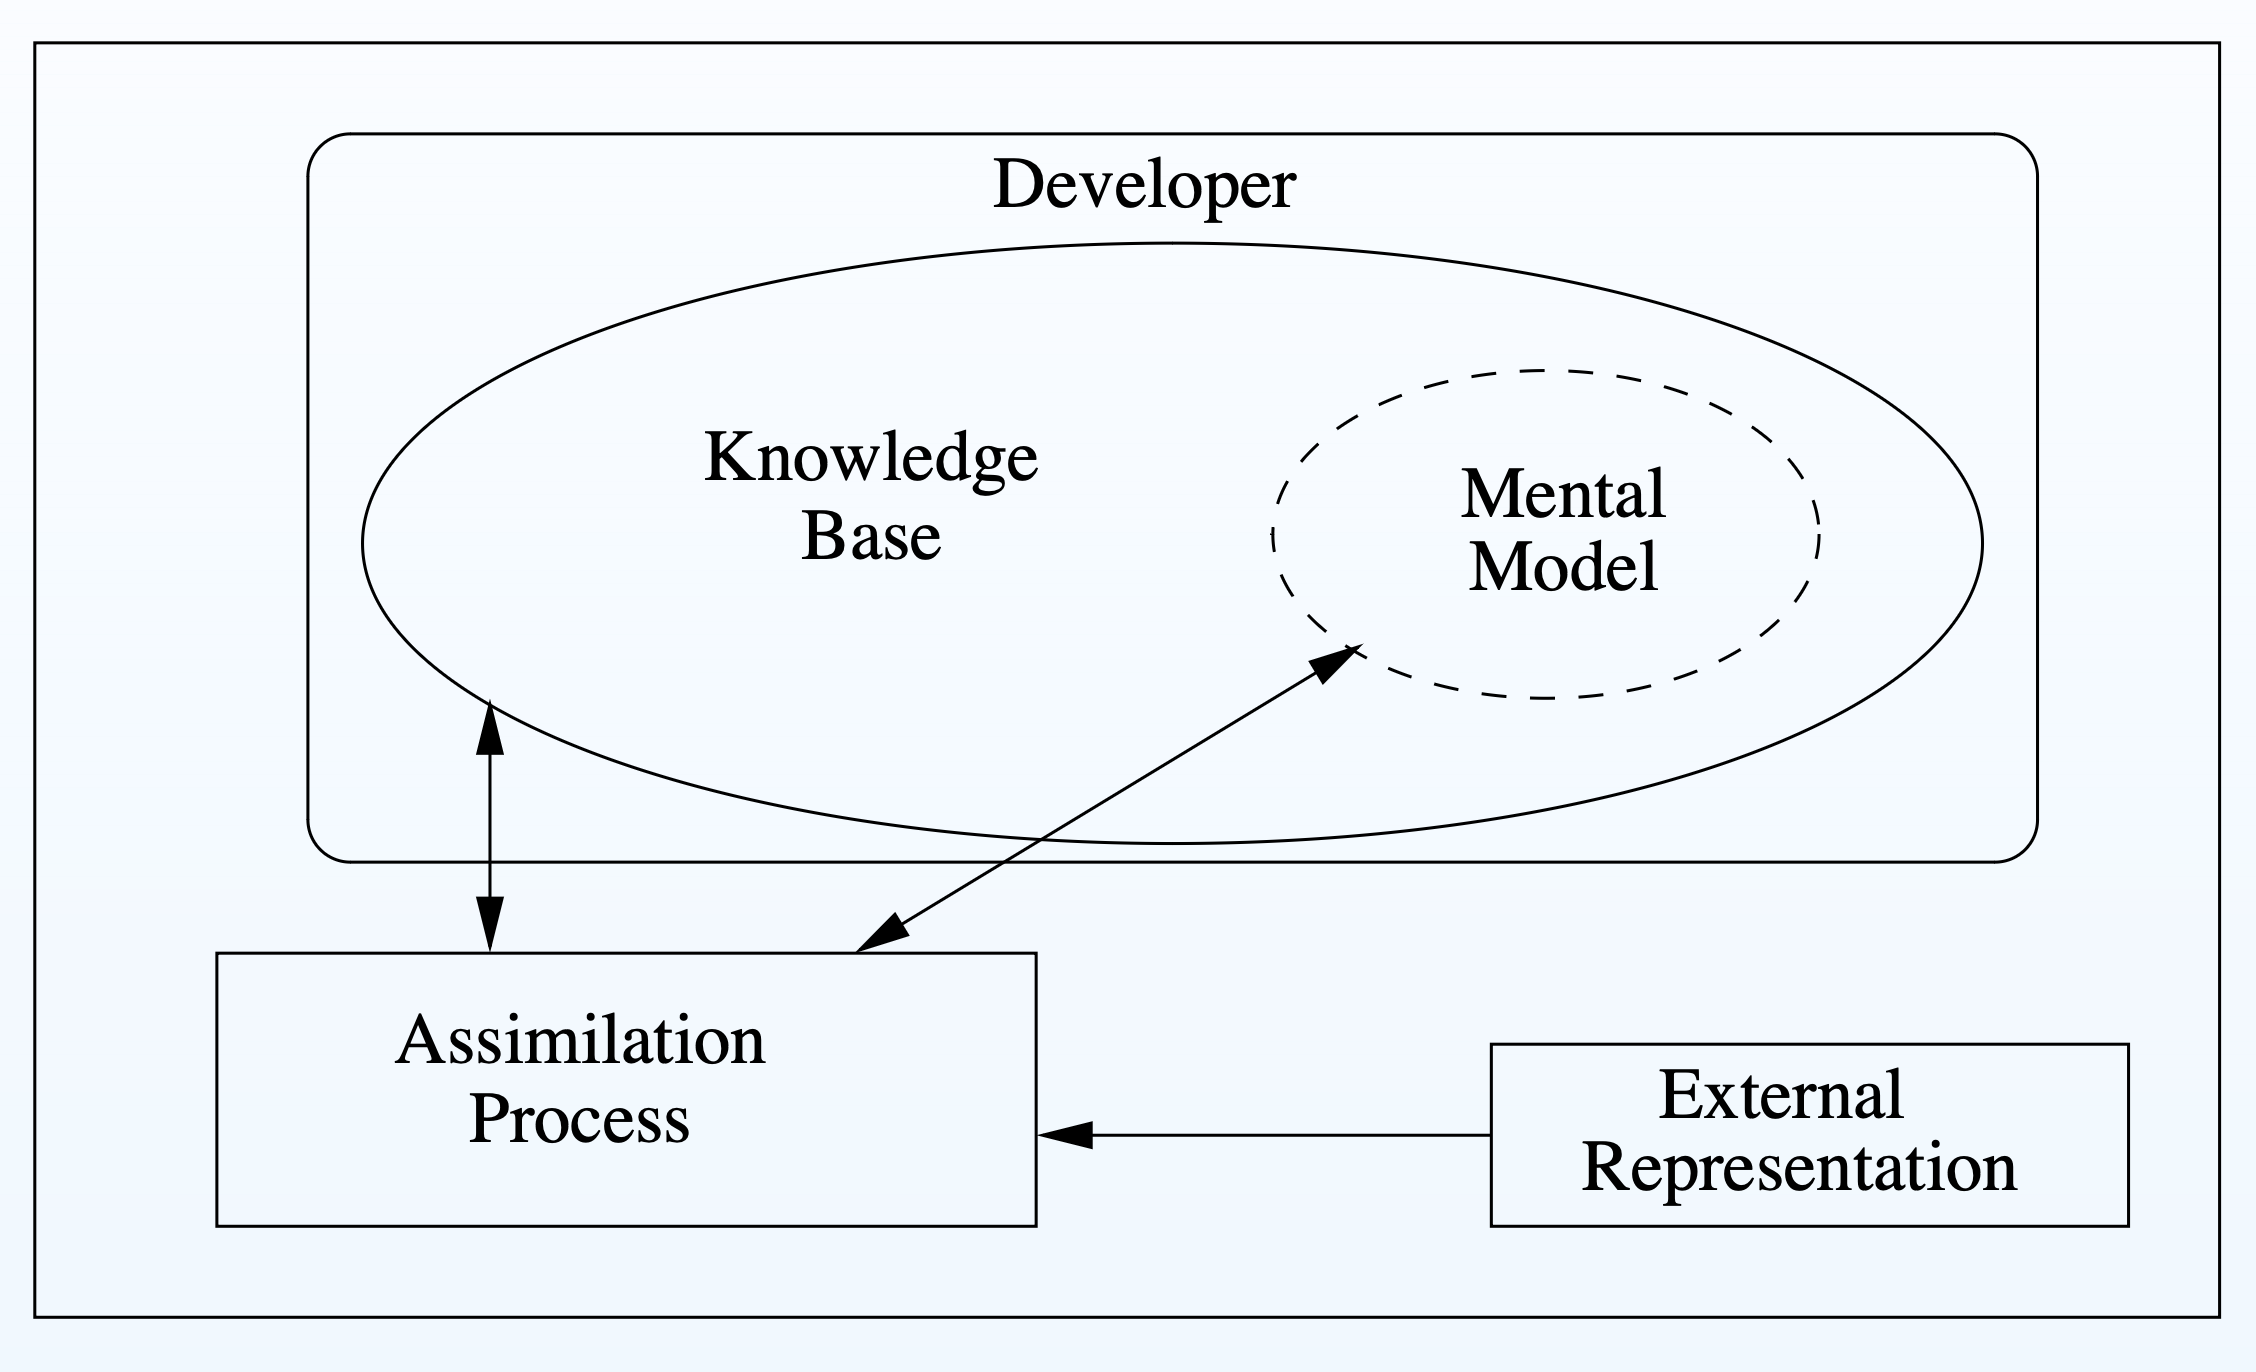
\includegraphics[width=8cm]{res/PCM.png}
    \caption{PCM by Michael}
\end{figure}

\begin{itemize}
    \item External Representation: e.g. source code, docs, peers\dots
    \item Knowledge Base: relevant knowledge that developers have already known, e.g. programming lang, domain knowledge
    \item Mental Model: current understanding, e.g. know parts, hypotheses
    \item Assimilation Process(内化过程): how to use all information to update the mental model, e.g. generation and verification of hypotheses
\end{itemize}

\subsection{可理解性与维护的关系}
可理解性关乎于开发者如何有效和高效地理解代码,以便有信心地进行维护活动。代码的可理解性与其维护性是紧密关联的。代码越容易理解,维护成本就越低,从而提高了代码的长期可维护性。
要提高代码的维护性,我们需要确保代码更容易、更快速且花费更少的精力去理解。

\subsection{如何评估可理解性?}

\paragraph{理解的有效性(Effectiveness)与效率(Efficiency)}要解释对一个实现的理解的有效性和效率,可以通过理解模型来实现,特别是考虑到同化过程的效果。

\paragraph{同化过程的有效性与效率}它取决于从知识库 (KB)、心智模型 (MM) 和外部表示 (ER) 中获取信息的效率和有效性。

\paragraph{信息的来源和理解难度的关系}信息的位置或来源对于理解来说非常关键。信息在心智模型、知识库还是外部表示中,这决定了理解的难度。

\section{Alterability}
\paragraph{可变性}是在不引入缺陷或降低现有产品质量的情况下,对产品或系统进行有效地和高效地改变的程度。

\subsection{Change Cases}
\paragraph{更改案例}描述了系统的潜在新需求或对现有需求的修改。它们的目的是预测和捕捉可能的更改,并指导系统的实现方式,以降低如果需要进行这些更改时的成本。

它们包括案例发生的可能性(Liklihood)和潜在的影响程度(Impact),可以视为系统演进的“用例”。

\subsection{评估可变性}
首先,需要确定实现应当适应哪些更改案例。
其次,针对这些更改案例评估实现。这意味着要查看系统或产品如何响应或适应这些特定的更改案例。

但请注意,有效和高效 "不包括与理解相关的成本
有些代码可能 "难以 "理解,但 "易于 "更改
因此,在评估可更改性时,应假设心智模型是 "完整的"(只要这样做是合理的)。

当一个更改案例的可能性较低时,它对可变性评估的影响也将较小。换句话说,如果预期某种更改的可能性非常小,那么在可变性评估中,我们不太需要考虑这种更改。当一个更改案例的影响较低时,它对可变性评估的影响也将较小。这意味着即使某种更改发生了,但如果其对系统或产品的实际影响较小,那么在考虑可变性时,我们不需要过于担心这种更改。我们应该主要关注那些\textbf{具有高可能性(Liklihood)和高影响(Impact)的更改案例},因为这些更改案例对可变性的影响最大。这意味着在设计和评估系统时,我们需要确保系统可以容易地适应这些具有高可能性和高影响的更改。

\subsubsection{评估影响}
对需求评估影响,而非现有代码。当评估更改的影响时,重点应该放在如何满足新的或修改后的需求上,而不是现有代码需要做多大的修改。影响是由现有系统的行为由于更改案例而改变的程度来决定的。例如,仅仅改变符号不会显著影响现有的行为,但改变游戏玩法会带来很大的差异。由于多种因素,评估更改的影响可能具有主观性,因此,可能难以为其提供一个精确的量化值。一种可能的方法是考虑你为这个更改案例准备支付的“原始成本”的比例。这种“成本”可以用财务、时间、努力或其他方式来衡量。通过这种方法,可以根据改变的大小和复杂性为其设置合理的预期。

\subsection{改变的位置和工作量}
在一个给定的更改用例中,对单个类中的代码进行所有必要的更改可能比在多个类中进行更改要容易。
原因:除了更改代码所需的时间,还有在不同类之间切换的时间。在类之间切换增加了出错的可能性。
在一个类中的单个方法中进行所有必要的更改可能比在同一个类的多个不同方法中进行更改要简单。
原因:再次涉及到在方法之间的切换时间。
在方法中更改一个语句可能比更改多个语句要简单。
原因:再次是因为切换。

进行“简单”的更改可能比进行“复杂”的更改要少工作。
例如,在switch语句中添加一个新的分支(该分支只对其他分支进行了简单的变种),与更改循环条件中的表达式相比。

\subsection{总结}
总之,可变性不是绝对的。软件或系统的可变性不是一个恒定或固定的属性。根据所需的更改类型,软件或系统的可变性可能会有所不同。

变更案例为评估可变性提供了一个方法,用于明确定义和描述可能需要对系统或软件进行的更改。它不仅描述了更改的具体内容,还可能包括更改的可能性和潜在影响。变更案例为评估和计划软件或系统的可变性提供了一个结构化的方法。这有助于确保可变性不仅基于直觉或主观判断,而是基于明确、详细和可衡量的标准。

一般来说,我们需要更改现有代码的次数越少,设计的可修改性就越高。
我们需要处理的地方越少(Efficiency)。
出错的可能性越小(Effectiveness)。

\section{Testability}
\paragraph{可测试性}测试性描述了为系统、产品或组件建立测试标准的有效性和效率,以及为确定是否满足这些标准而执行测试的能力。如果一个系统的测试性高,那么开发团队可以更轻松地定义测试标准,并验证系统是否满足这些标准。这可以确保软件的质量并减少缺陷。
\paragraph{测试}的主要目的是识别软件系统中的错误、缺口或未实现的需求。通过测试,开发者可以确保软件系统满足特定的测试标准或需求,从而确保产品的质量和稳定性。

根据测试标准(如性能、可用性、功能性)的不同,存在不同类型的测试。
系统测试:测试整个系统,确保所有部分和功能都按预期工作。
集成测试:确认独立开发的子系统能够协同工作。它关注的是接口和交互点,确保子系统之间没有冲突。
单元测试:针对单一的子系统或组件(如单个类)进行的测试。它通常关注特定功能的正确性。

手动测试涉及实人执行特定的测试用例,而自动测试使用脚本或其他工具自动执行测试。虽然手动测试在某些情况下可能更为直观和灵活,但自动测试通常更高效,尤其是对于需要频繁重复的测试。

测试涉及执行想要测试的代码,即被测实现(Implementation Under Test, IUT),并检查IUT的行为是否如预期。由于软件可能在各种条件下运行,因此需要在不同的条件下进行测试。这通常意味着为IUT提供不同的输入。

\paragraph{测试用例}是一组操作,通常由一组输入指定,对IUT执行以确定其是否导致正确的行为。

测试用例规定内容:
IUT:指定要测试的代码或模块。
预测试状态:这是执行测试之前IUT应处于的状态。
输入:要应用于IUT的数据。
预期状态或行为:这是在给定输入的情况下IUT预期的行为或输出。
执行测试用例的步骤:
预测试状态设定:确保IUT处于正确的预测试状态。
提供输入:根据测试用例的指定,为IUT提供输入数据。
执行IUT:使用给定的输入运行IUT。
结果验证:将IUT的实际行为与预期行为进行比较。这一步是判断测试是否通过的关键。

良好测试用例的一些关键属性超越了基本的“提高检测缺陷的概率”。为了确保软件的质量和可靠性,设计和执行高质量的测试用例是至关重要的。快速(Fast):
效率:快速的测试用例可以在短时间内执行,这意味着可以更频繁地运行它们,从而更早地检测到潜在的问题。
意义:如果测试用例执行速度快,那么在持续集成和持续部署的环境中,它们更有可能被频繁运行,这有助于提早捕捉和修复缺陷。
独立(Independent):
有效性:如果测试用例之间存在依赖关系,那么测试用例的执行顺序可能会影响结果,从而增加了出错的概率。
效率:
理解依赖关系需要额外的时间和努力。
如果某些测试用例依赖于其他测试用例,那么在执行特定测试之前,可能需要先执行其他测试,从而增加了测试的总体时间。
简单(Simple):
有效性:简单的测试用例降低了设计和执行出错的可能性。
效率:简单的测试用例往往执行速度更快,并且更容易理解,这也可能增加了测试用例的独立性。
可重复(Repeatable):
有效性和效率:
可重复性确保每次运行测试用例时都使用相同的预测试状态和固定输入,从而保证了一致性和可靠性。
这意味着测试用例的结果在不同的执行之间是一致的,从而提高了测试的准确性。

手动测试比自动化测试花费更长的时间,导致效率较低。由于手动测试时间较长,常常有将多个测试组合在一起的倾向,从而降低了测试的独立性和简单性。这可能会导致难以确定特定的缺陷来源和复杂的测试逻辑。手动测试的可重复性较低,因为执行每次测试时可能会有些许的变化,如人为错误、不同的执行顺序等。自动化测试在初始阶段可能会有较高的设置成本,但一旦建立起来,其后续成本就会降低。相反,手动测试的成本随着时间而持续累积,因为每次都需要人工介入。

自动化测试工具:
单元测试:
这是最基本的测试层级,针对代码的小部分(如一个函数或方法)。
工具:目前有很多“X-Unit”测试框架可用,例如JUnit(Java环境中的单元测试工具)。
集成测试:
测试多个子系统或组件是否能正确地一起工作。
工具:有一些工具可以用来进行集成测试,例如Mock测试工具,它可以模拟部分系统来进行集成测试。
系统测试:
测试整个系统的功能和性能。
工具:通常为特定系统定制,因为它涉及到完整系统的全面测试。

\paragraph{测试标准}是一组规则,这些规则定义了测试用例集(或称为测试套件)必须满足的要求,以便实现正在测试的(Implementation Under Test, IUT)被视为可接受的。测试标准提供了一个明确的、可衡量的方法,以确定系统、组件或功能是否满足预定的质量标准或要求。它们是质量控制过程中的关键组件,帮助确保软件产品的质量、性能和可靠性。

\paragraph{分支覆盖率}是一个常用的软件测试标准,要求在测试套件中的至少一个测试用例执行IUT中的每一个分支。这确保了代码中的每一个决策路径都被测试过,从而提高了发现潜在缺陷的可能性。

\paragraph{测试用例}是对如何测试特定功能或条件的明确规范,它通常包括前置条件、输入、期望的输出以及后置条件。

一个私有方法,这意味着它不能被类外部的代码直接访问。这对测试来说是一个问题,因为直接测试私有方法通常较为困难。测试人员需要找到一个方法来间接地测试它,例如通过一个公共方法。这会增加测试的复杂性。分支覆盖率要求每一个代码分支都至少被执行一次。这就需要为它的调用者方法选择适当的输入值,以确保方法中的每一个分支都被触发和测试。
这是一个复杂的任务,因为你需要深入了解代码的工作方式,以及哪些输入会触发哪些分支。

将方法从私有更改为公共可能会暴露类的内部细节,从而增加代码的脆弱性或违反面向对象设计的原则。

如果测试结果需要手动检查,那么这个过程会非常繁琐,并且效率低下。
手动验证测试结果也更容易出错,因为人们可能会遗漏某些细节或误解预期的行为。

\subsection{提高测试性}
测试的主要目的是为了模拟各种输入,观察并验证输出结果是否满足预期。为了实现这一目标,我们需要确保软件或系统的控制性和可观察性。

\paragraph{控制性 (Controllability)}涉及到我们能够如何控制或操作一个系统、组件或功能的能力。换句话说,我们需要能够按照我们想要的方式提供输入或触发条件。提高控制性意味着要确保测试人员或测试工具能够轻松地为软件或系统提供预期的输入或条件。

\paragraph{可观察性 (Observability)}
涉及到我们能够观察或看到一个系统、组件或功能的实际行为或输出的能力。为了有效地进行测试,我们需要能够清晰地看到软件或系统的行为,以便与预期的结果进行比较。
提高可观察性意味着确保输出、日志、状态或任何其他与软件或系统的行为相关的信息都是可访问和可理解的。

\subsubsection{设计上的实现}
如果系统具有结构化和功能明确的类,则测试者可能会更容易地控制和观察系统的各个部分。类的粒度和职责划分对于控制性和可观察性都至关重要。如果一个类提供了功能明确、有用的公共方法,那么它的行为和状态将更容易被控制和观察。公共方法为外部提供了与类交互的接口。选择合适的类和方法可以显著提高系统的测试性。开发者需要仔细选择和设计类及其方法,以确保它们对测试活动有利。

虽然增强控制性和可观察性是有益的,但过度的控制性和可观察性可能会导致其他问题。例如,过度的可观察性和控制性可能会破坏封装,从而增加系统的复杂性和引入潜在的错误。

\subsection{总结}
要提高系统或软件的测试性,一个关键策略是提高其控制性和可观察性。当这两个方面都很好时,测试过程将更加顺畅,能够更容易地识别和定位问题。
